\documentclass{scrartcl}

%Packages
\usepackage[utf8]{inputenc}
\usepackage[english]{babel}
\usepackage{graphicx}
\usepackage{wrapfig}

\title{Team Faabs - Technical Paper}
\author{Fabian Brune, Mark Krause, Jurij Lenz}
\date{May 2023}

\begin{document}

\maketitle


\begin{figure}[h]
    \centering
    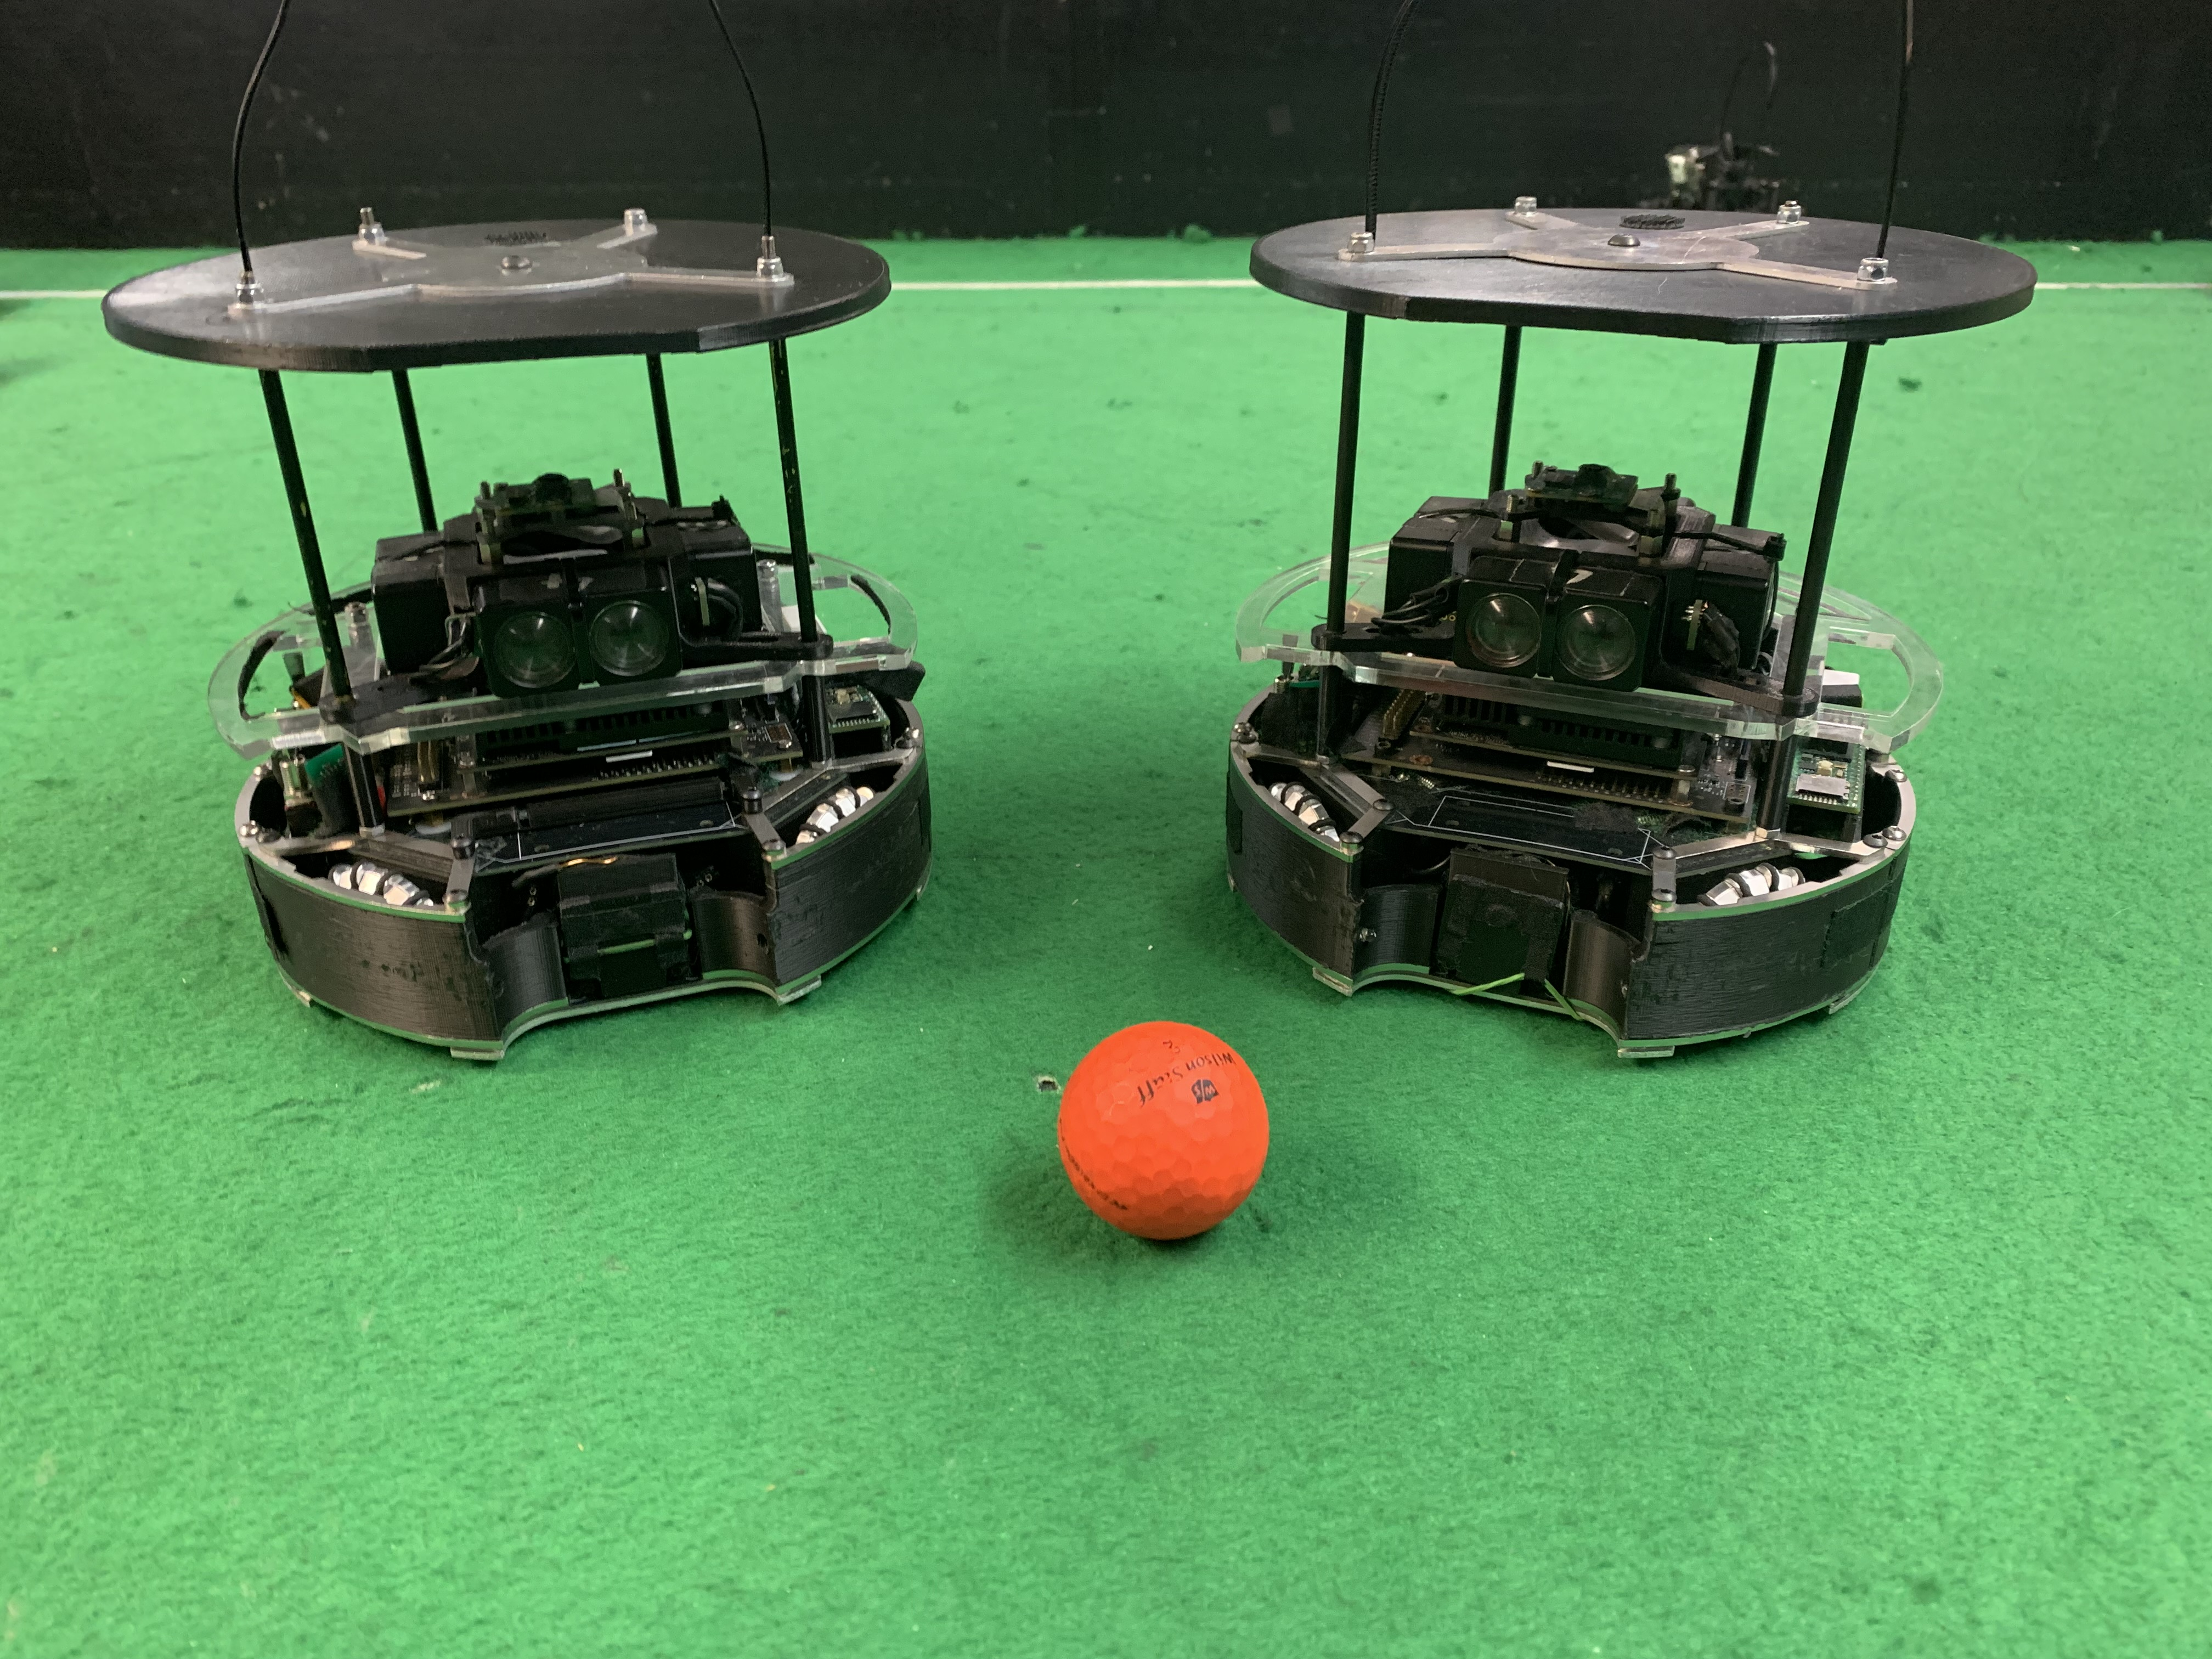
\includegraphics[width=\textwidth]{img/Roboter mit Ball querformat 2.jpg}
    \caption{Team Faabs - Fabian Brune, Mark Krause, Jurij Lenz}
    \label{fig:team}
\end{figure}


\newpage


\tableofcontents
\newpage


%Team general
\section{introduction}
\subsection{Team}


In our Team, everyone has a specific task to do.
\begin{enumerate}
    \item{Mark Krause: Software and circuit design }
    \item{Fabian Brune: Hardware design }
    \item{Jurij Lenz: Raw Hardware }
\end{enumerate}

\begin{figure}[h]
    \centering
    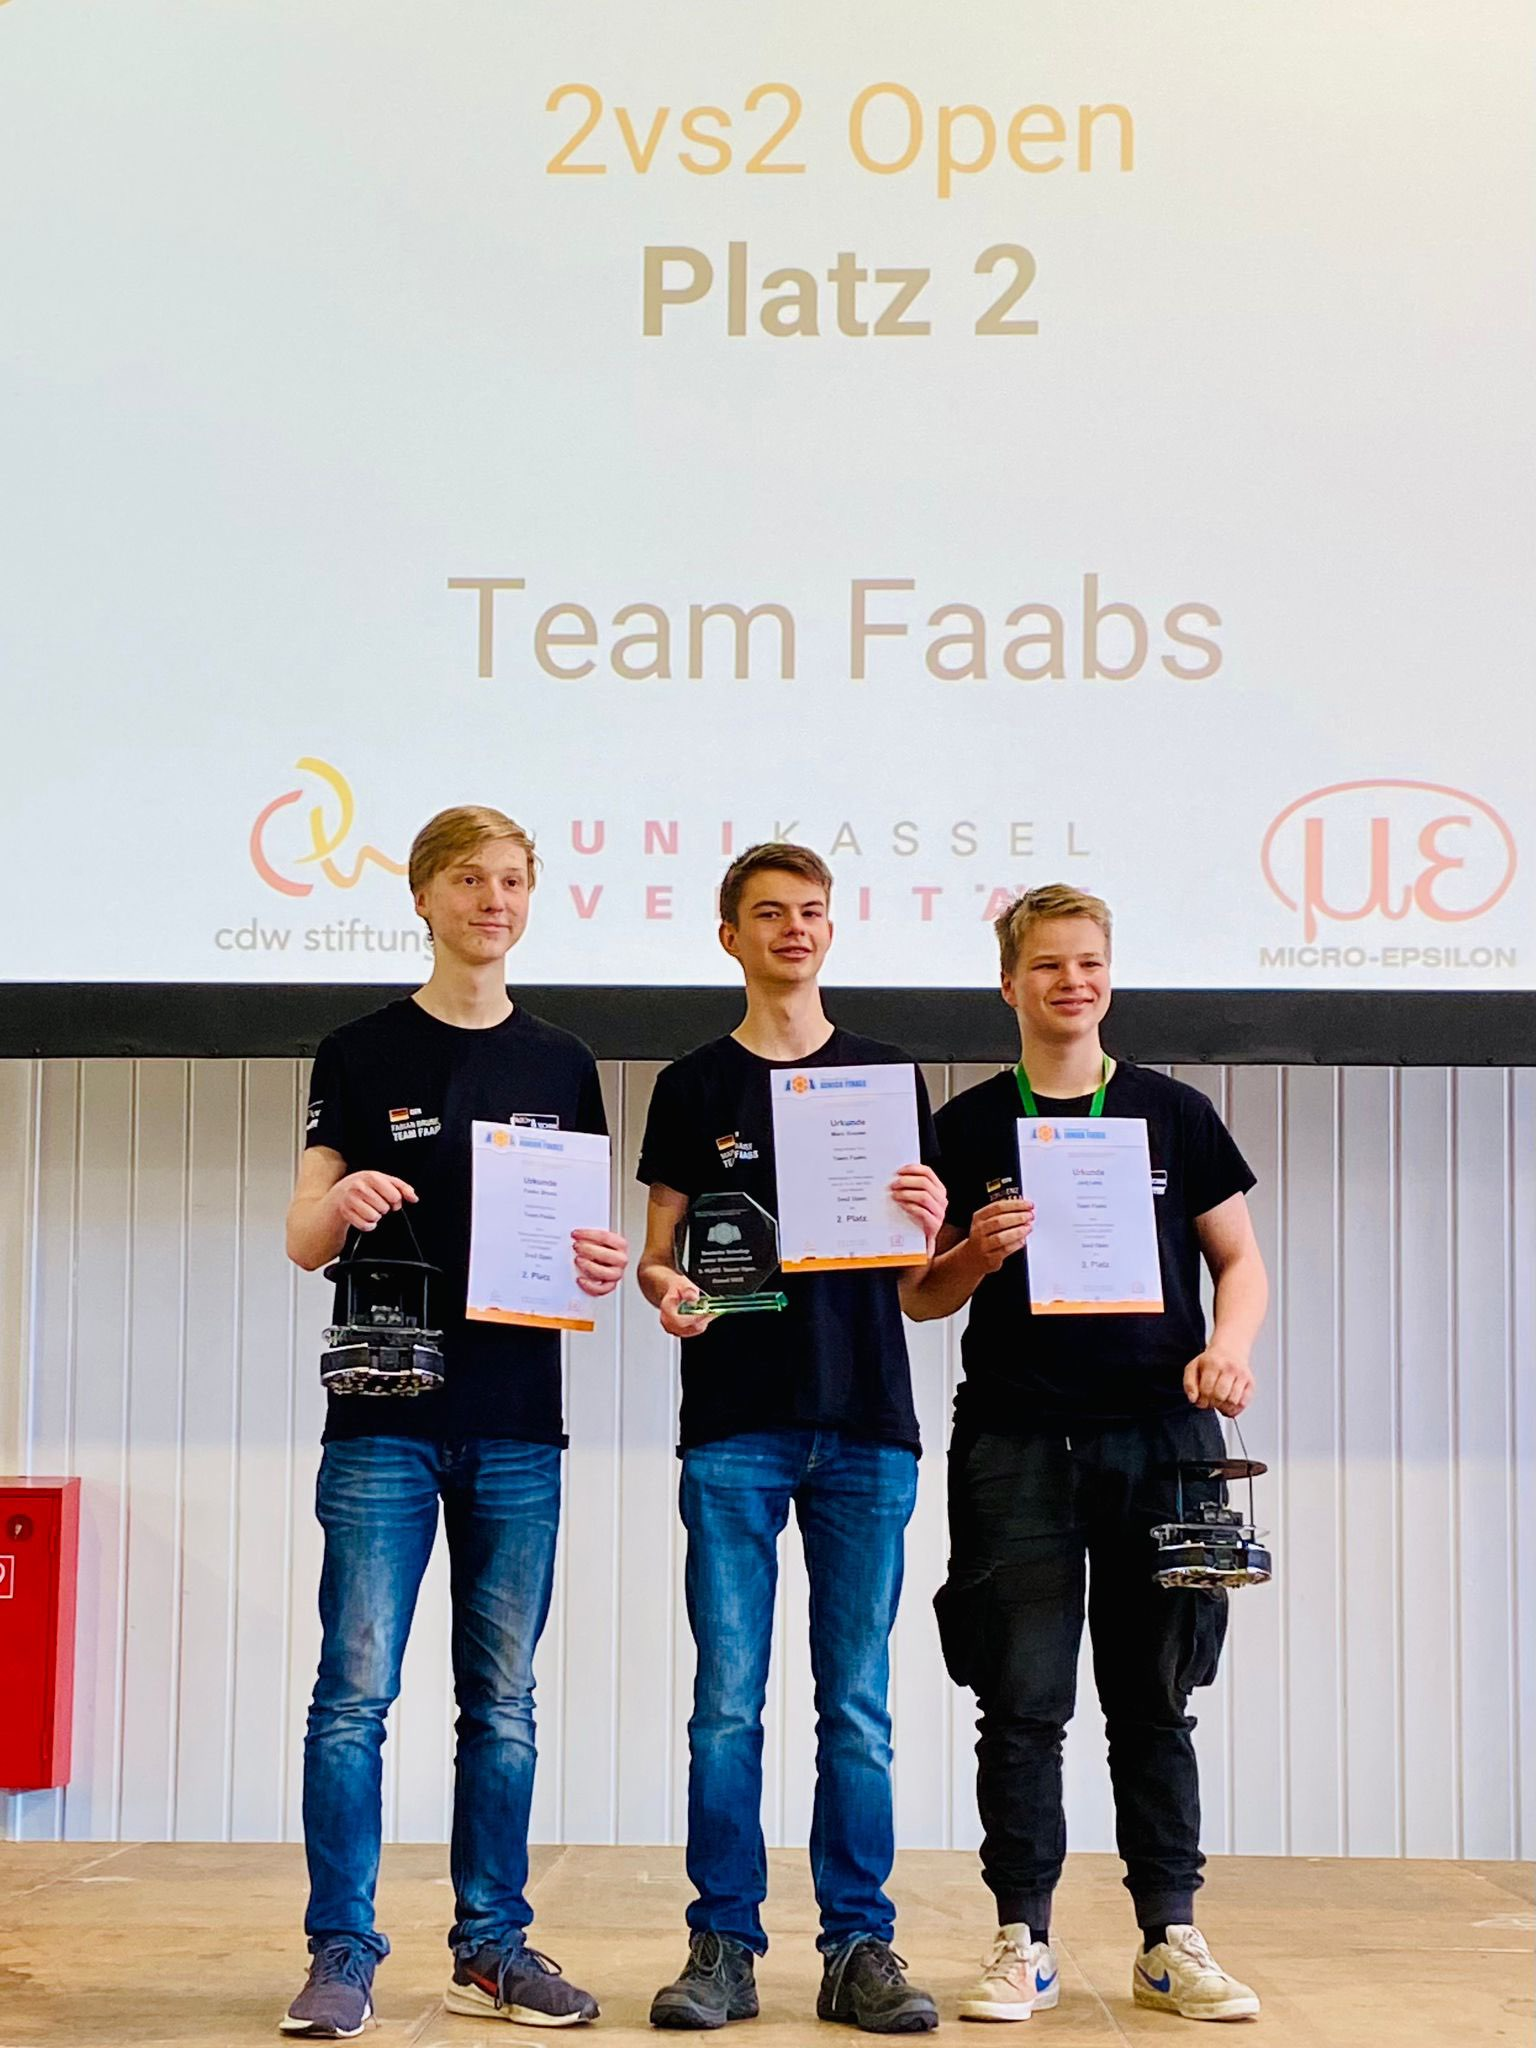
\includegraphics[width=0.75\linewidth, ]{img/Siegerehrung Kassel 1.png}
    \caption{Team Faaaabs - Fabian Brune, Mark Krause, Jurij Lenz}
    \label{fig:team}
\end{figure}

\newpage

\subsection{School}

The Robotics program of our school was created 2011. Since then, we managed to win the World Open
multiple times in either Soccer LightWeight, Soccer Open or OnStage.
We try to put our new teams as fast as possible in the top leagues. With the gathered experience, we always
have teams to follow our footsteps.
\newline
\begin{figure}[h]
    \centering
    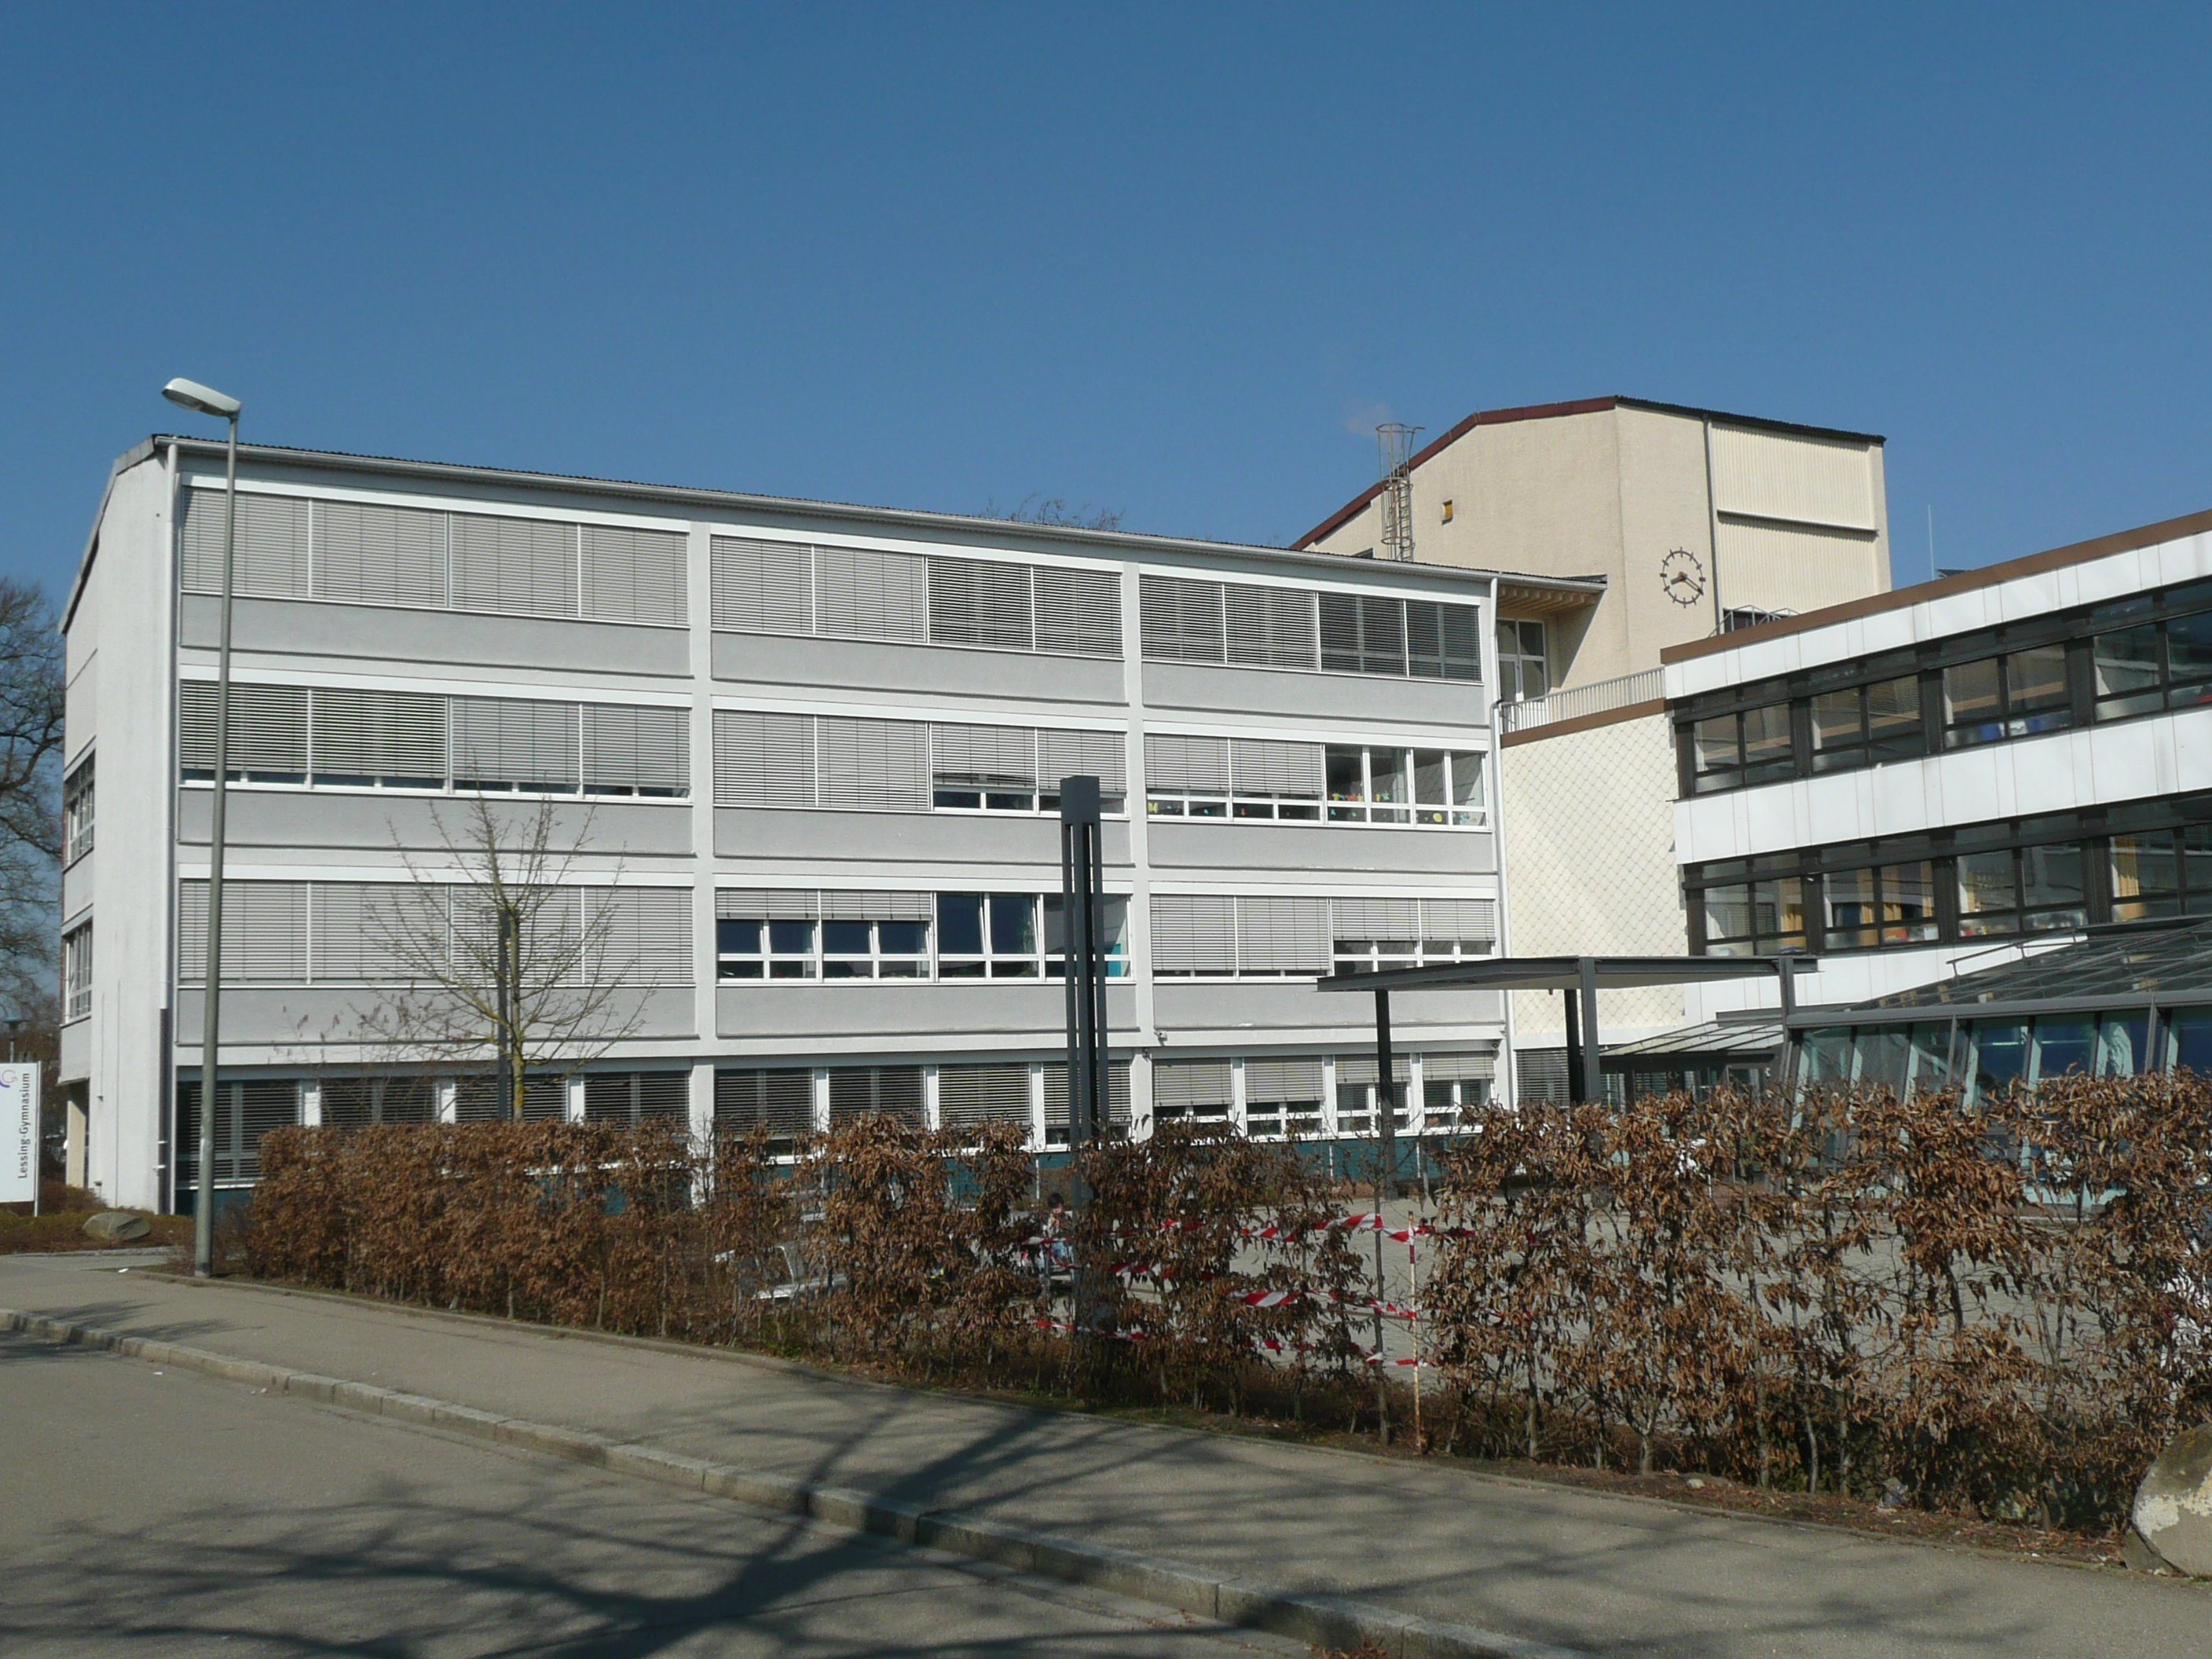
\includegraphics[width=\textwidth]{img/lgnu.png}
    \caption{LGNU - our school}
    \label{fig:lgnu}
\end{figure}
\subsection{Abstract}
We are a Team of three students from the Lessing Gymnasium Neu-Ulm in Germany. Furthermore, we founded our Team
in 2019 and first participated in the RoboCup Junior in 2019. Robotic is a big part of our daily life.
We meet on school days and even on weekends and holidays.

\begin{figure}
    \centering
    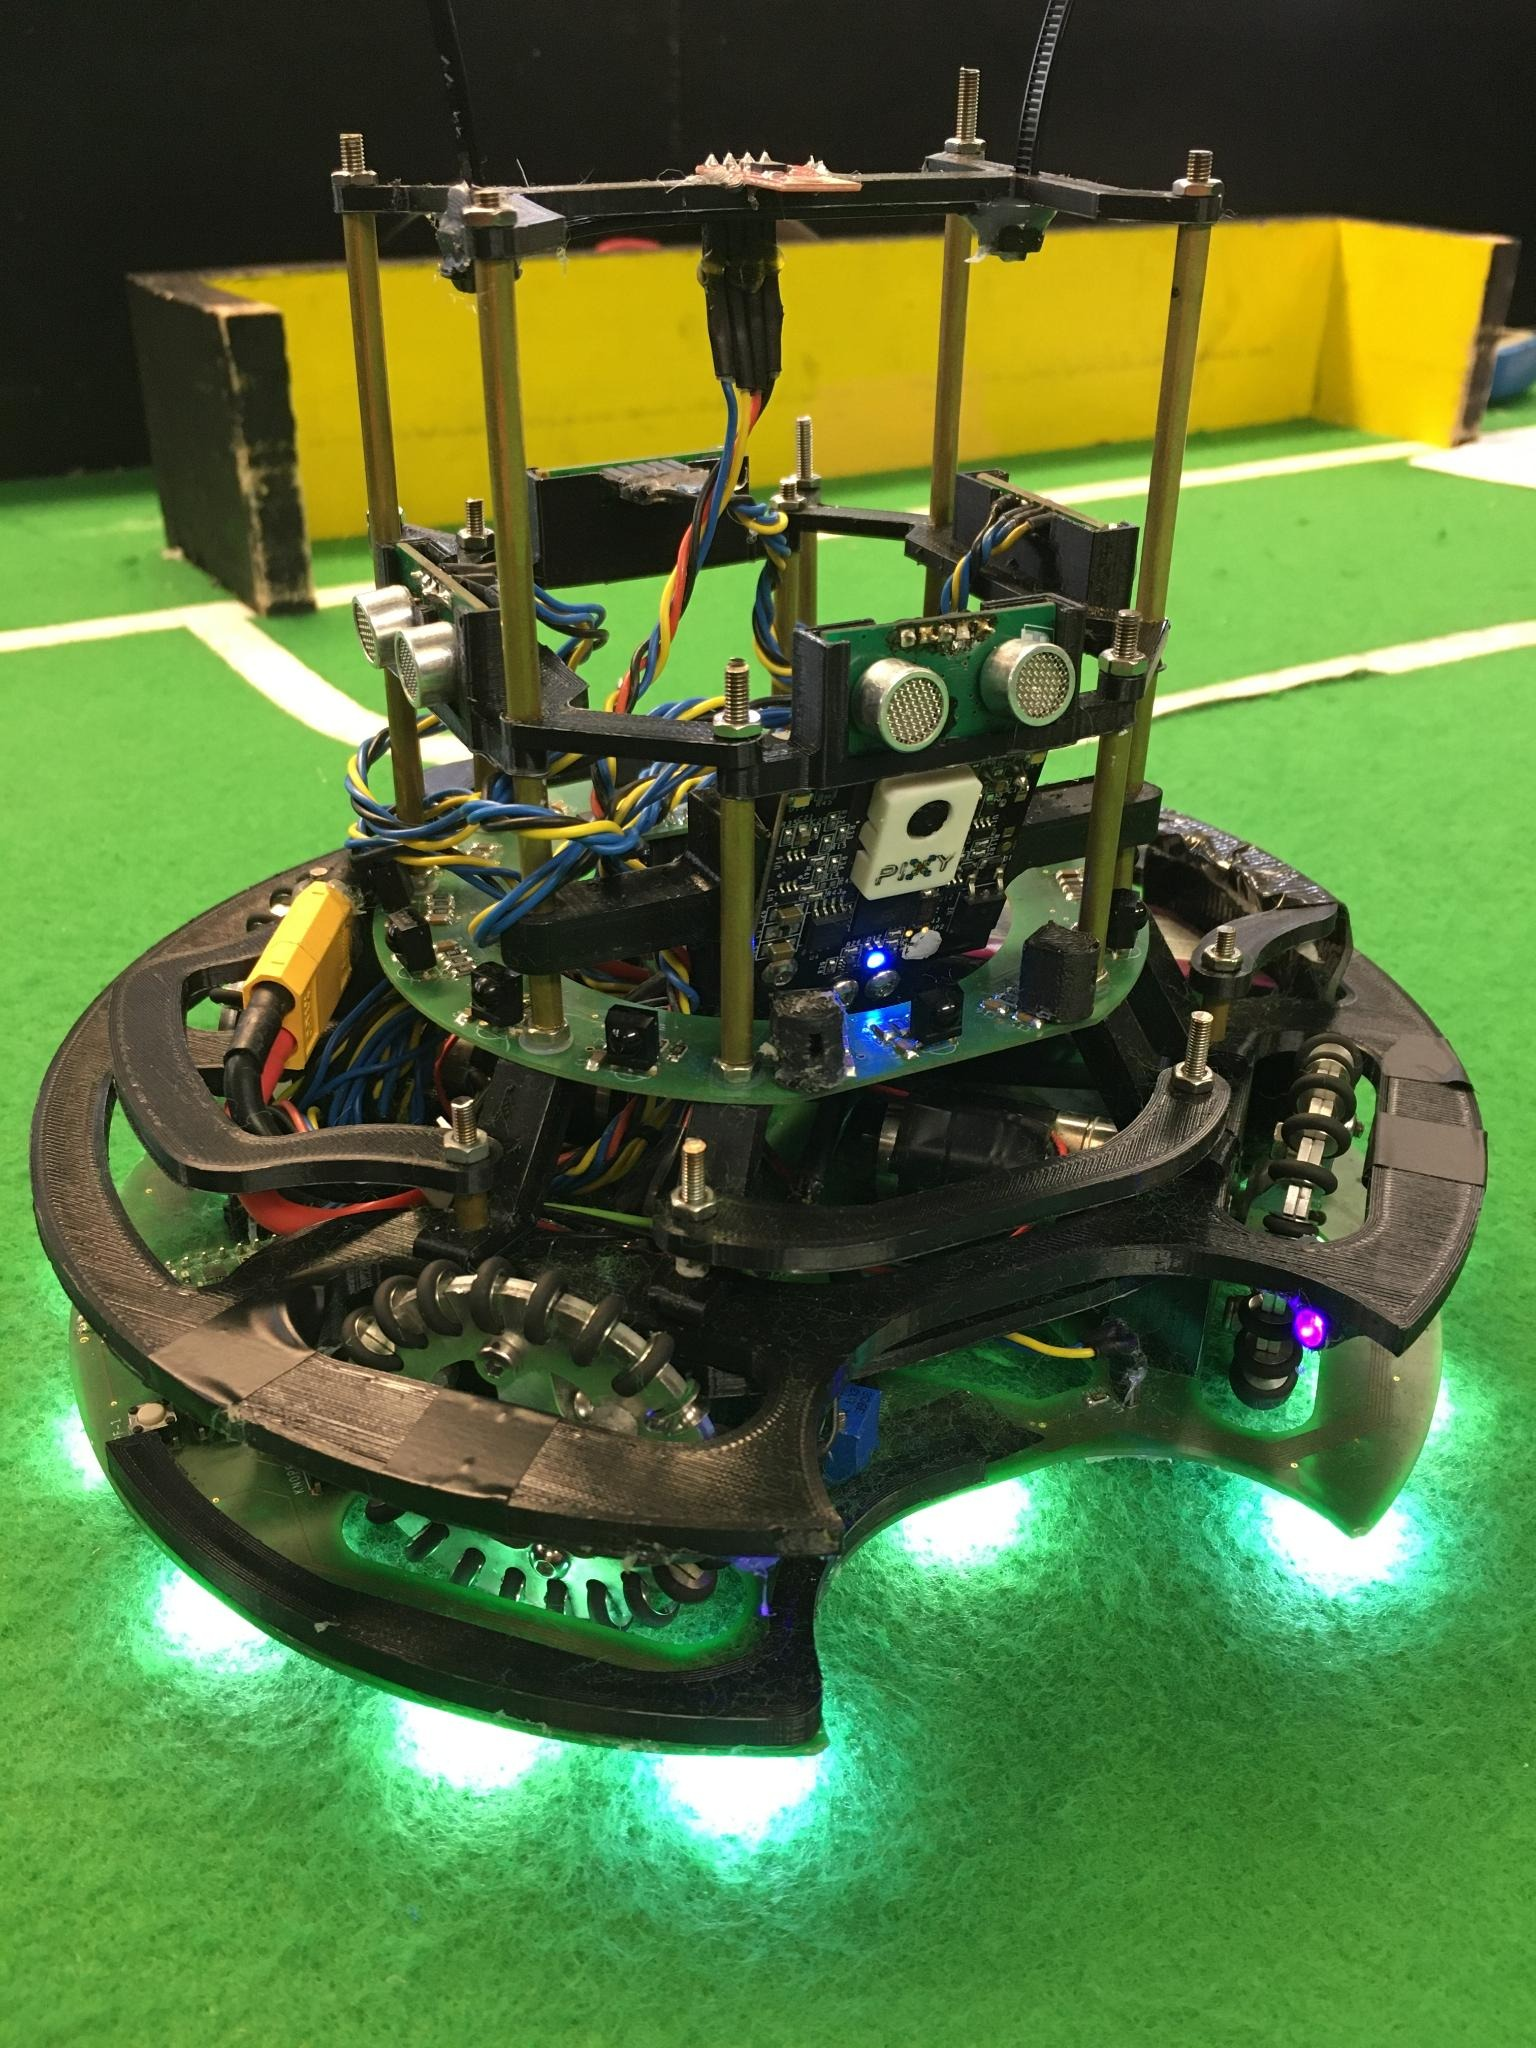
\includegraphics[width=\textwidth]{img/LWLBot.png}
    \caption{Robot from 2022 before the eruope open}
    \label{fig:LWLBot}
\end{figure}


%\newline
%\newline
We started developing our Robots in mid 2022 and had a first Prototype in late 2022. After final design
choices, we had our Robots for the German South-Open in early 2023. From this point on, some progress was
made in the Hardware sector.
After optimizing our program, we managed to reach the second place.
\newline
After the South-Open we redesigned our kicker and continued fixing small hard-\& software problems. We discovered, 
instead of using a bad dribbler, just to dont use one at the German Open, because it worsend our movement with the ball .
With these improvements we managed to gather the second place at the German Open and qualified for the World Championship.

\section{Development \& Testing}

\subsection{Development}
Due to the pandemic we weren't able to get much experience. In 2022 we had our first real RoboCup
in the LightWeight International League where we got second at the European Championship. With this experience we started to design the 2023 Open Robot.
\newline
The design of our robots aims to be as rigid as possible, while keeping the robot manouverable.
To achieve this goal, we used metal and 3D printed Parts in combination with optimised circuit boards.
With our Software, we are able to travel with high speeds to the ball use our dribbler and
hit a goal without going out of bounce (most of the time).

\begin{figure}[!h]
    \begin{center}
    \resizebox*{0.4\columnwidth}{!}{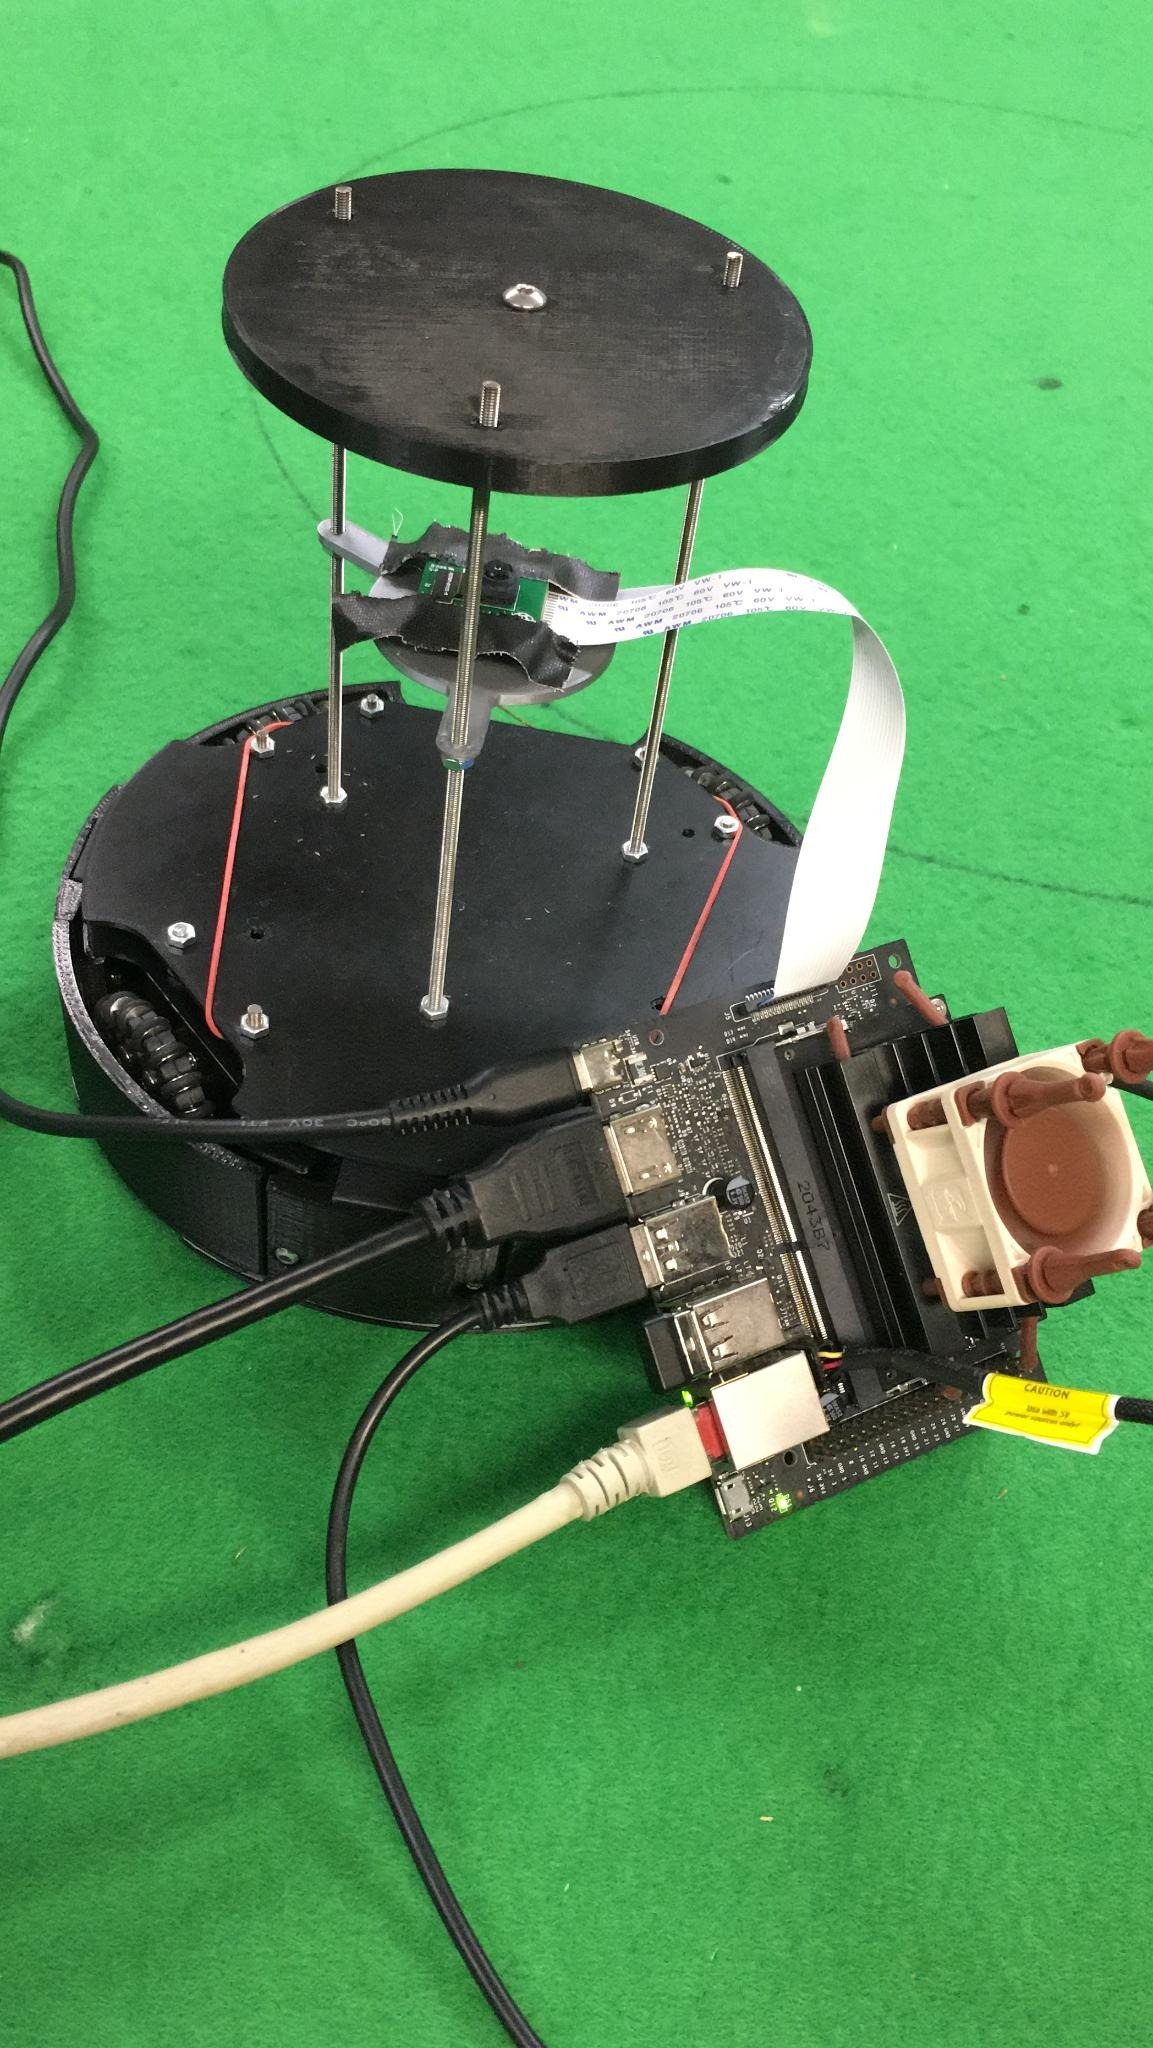
\includegraphics{img/prototype.png}}
    \caption{prototype from december last year}
    \label{prototype}
    \end{center}
    \end{figure}

\subsection{Mechanical Design}
All our parts were designed using 'Autodesk Inventor 2023 Professional' and 'Autodesk Eagle 9.6.2'.
Most of our parts are printed with our Prusa MK3S+ and the metal parts are produced
by our sponsor "Blech und Techhnik".

\begin{figure}[!h]
    \begin{center}
    \resizebox*{0.5\columnwidth}{!}{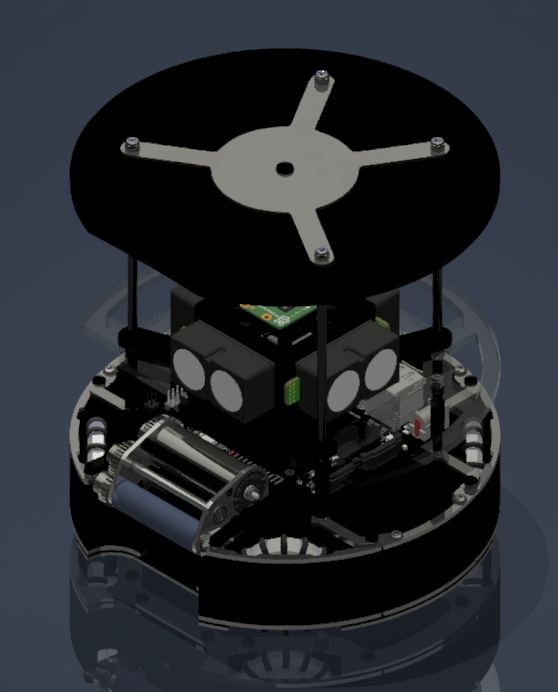
\includegraphics{img/Roboter Home.png}}
    \caption{CAD design createt by Fabian Brune (last updated 25.6.23)}
    \label{Robot}
    \end{center}
    \end{figure}

Traveling with high speeds, while being strong is also a huge challenge. To achieve this, we use high quality
Maxon DC Motors in combination with the VNH3SP30 driver chip. To put the force on the ground, we designed
new Omniwheels
The OmniWheel consists of two independent aluminum pieces screwed together. For the small wheels we use a small
aluminum piece covered with an O-Ring out of EPDM plastic.
\newline
To protect this whole construction from the opponent robot, everything is moved into the robot and a 3D
printed and metal protectors are covering the whole inner side of the robot~\ref{fig:Roboter}..
\newpage


\subsection{Electrical Design}
To detect various elements and control the whole robot we use a Teensy 4.1 microcontroller and a jetson nano
for ball detection. All electronic parts are soldered to circuit boards.
\newline
We have a total of four Circuit Boards:
\begin{enumerate}
    \item{Line Detection\& motordriver PCB}
    \item{camera\&lidar PCB}
    \item{Controller PCB}
\end{enumerate}
Each Circuit Board has a predetermined task and all the above are controlled by the Teensy 4.1
and the Jetson Nano 2Gb.

We order our Circuit Boards from a local company and solder the parts manually on the boards.

\subsubsection{Line Detection\& motordriver PCB}

%\begin{wrapfigure}{r}{4cm}
% \centering
% \includegraphics[width=0.75\linewidth]{img/eagle/LineDedectionPCB.png}
% \caption{PCB}
%\label{fig:LDPCB}
%\end{wrapfigure}

The Line Detection PCB consists of a circle with a cross of phototransistor pairs, our motordrivers and the kicker control . To connect all
48 sensors to our main controller, we use analog multiplexer. The multiplexers are switched parallel
to save ports.
\newline
As you can see on the right, we use pairs of two phototransistors and one led. For us, this is the
best way to detect the line.

\subsubsection*{camera\&lidar PCB}
On this very small and special PCB, we combine our most important sensor, the lidars~\ref{lidars} and our raspery pi
cam. The camera is used for ball and goal detection. It is directly programmed on our Jetson in OpenCv.
Our lidars are conected to the Teensy 4.1 on the Controller~\label{PCB:Controller} PCB via I2C.

\begin{figure}[!h]
    \begin{center}
    \resizebox*{0.49\columnwidth}{!}{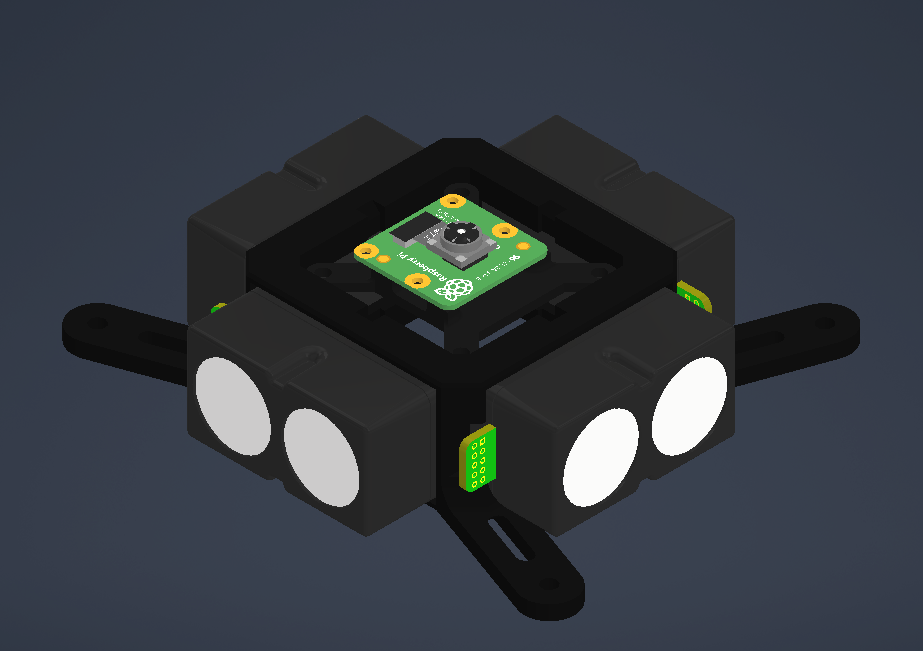
\includegraphics{img/LidarBaugruppeNormal.png}}
    \caption{lidars}
    \label{lidars}
    \end{center}
    \end{figure}


\subsubsection{Controller PCB}

On our controller PCB we got the most imortant parts of our Robot like the Nvidia Jetson Nano 2gb Developer Kit
and the Teensy 4.1. Our dribbler is also located on our main PCB. We use our dribbling device
to give the ball a backspin, so that it stays right infront of our kicker. You can also find our baterry packs
and a diod.

\subsection{Software} 
As we all know, that's the objective:
\begin{enumerate}
    \item{Approach the ball quickly and precisely to get it into the ball pit.}
    \item{Aim for the goal as quickly as possible, while ball is save.}
    \item{Score as fast as possible.}
    \item {stay inside the playing field very consistently}
\end{enumerate}
Accordingly, a modularization of the code can be set up.
\subsubsection{Object detection}
We detect the orange ball, the yellow and the blue goal. This is done with the open-source computer vision library "OpenCv" (v4.1.1)
on our jetson nano. We also do multithreading to achieve this three detection processes parallel with the lowest latency possible.
Our resolution is 816 on 616 pixels in one frame.
\subsubsection{Onrobot communication}
The Jetson programms and talks to the Teensy via an usb cable and a raw HID interface. This proofed very stable and fast. The Teensy decides where
to drive because its receives all sensor data.

\begin{figure}[!h]
    \begin{center}
    \resizebox*{0.4\columnwidth}{!}{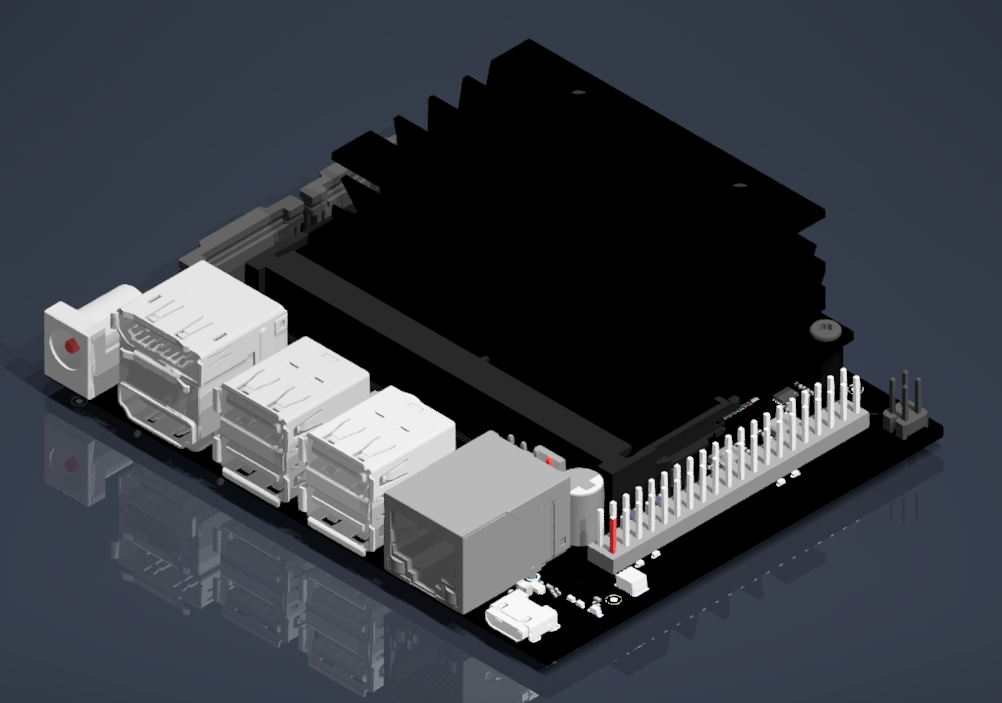
\includegraphics{img/Jetson.png}}
    \caption{Jetson Nano}
    \label{jetson}
    \end{center}
    \end{figure}

\newpage

\subsubsection{Ball approach}
In our understanding, to achieve a good base for all soccer actions, it should be key factor to get the ball
consistently and fast into the ball capturing zone.
As we nearly always drive alined to the enemy-sided wall (to minimize the risk of scoring in our own goal) our
calculations follow the same pattern over and over again. As an input they get the x and y coordinate of the
ball, relative to the robots origin. As an output the algorithm generates a direction and a velocity where to drive.
Concretly we try to get a fix position realtive to the ball and move this point in a cone in front of the ball-capuring-zone.
As the ball is directly in front of the robot, it can just drive forward to get the ball in the dribbler. The biggest challenge is,
to calculate the optimal curve with direction and velocity vectors.

\begin{figure}[!h]
    \begin{center}
    \resizebox*{0.5\columnwidth}{!}{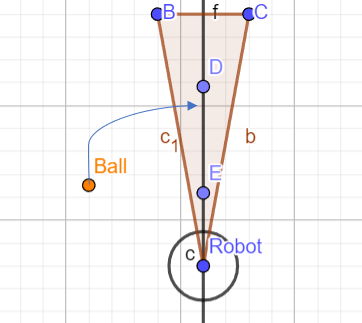
\includegraphics{img/ballaproach.png}}
    \caption{ballaproach}
    \label{balla}
    \end{center}
    \end{figure}
    
\subsubsection{Aiming at the goal}
To detect the goals we are also using our jetson nano. We only use the agles of the goals for the positioning on the field
and shoting in the right direction and not blind. The bot only shots when it is in range and good alined with the goal to minimize unnecessary ball losses.

\subsubsection{detecting the white lines and avoiding out of bounds}
To know where the Robot has to drive when it see the white line, it collects all coordinates of all linesensors that have seen the line in ableshort period of time
and calculate the opposite vector. In future we plan to update it, becaus it proofed very annyoing and not quiet a hundred percent secure.
Also we use our LIDAR Sensors to avoid to close wallcontacs on high velocities, which turns out really reliable and usefull.

\subsubsection{special tricks and gimmics (butch)}
In case that we don't see the ball on the field, we drive to fix points on the field to save some time driving to the next neutral spot.
Also we try to communicate if the ball is close to one robot via buetooth, so that the other one can drive to the back not disturbing the attacker.
We didn't want to have a set goalie, because of the fact that it may be more usefull to have two attackers.

\subsubsection{kicking device}
For our kicking device, we use 3Dprinted parts with an optimal design and a self wrapped coil, wich forces an iron bolt to move towards the ball.
With this technique we can transfer nearly all of the kinetik energy from the iron bolt to the ball. This allows us an direct
shot at the goalon the other side of the field.

\begin{figure}[!h]
    \begin{center}
    \resizebox*{0.5\columnwidth}{!}{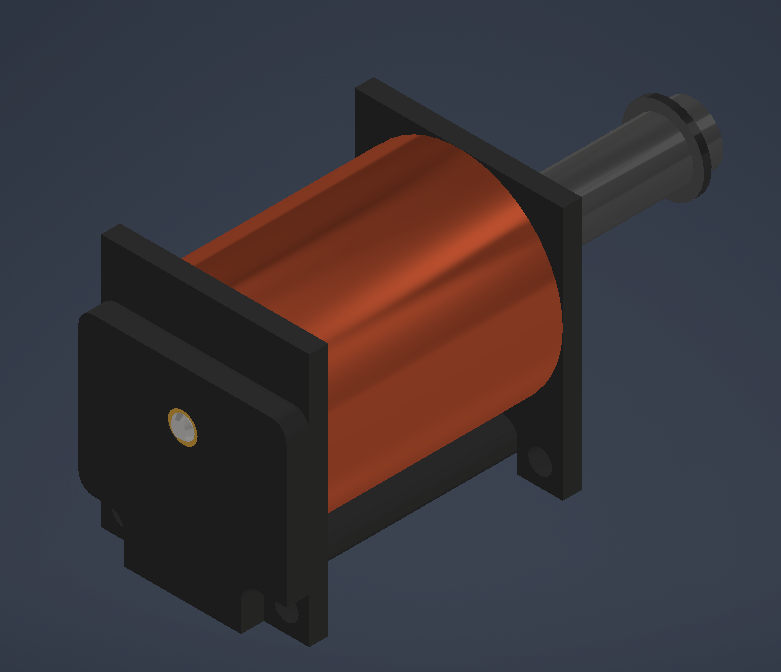
\includegraphics{img/Schuss.png}}
    \caption{kicker}
    \label{kicker}
    \end{center}
    \end{figure}

\section{Experience 2023}





\end{document}



